\documentclass[tikz,border=3.14pt]{standalone}
\usepackage{tikz}
\usetikzlibrary{arrows.meta}
\usepackage{amsmath}
\usepackage{physics}

\ExplSyntaxOn
\msg_redirect_name:nnn { siunitx } { physics-pkg } { none }
\ExplSyntaxOff

\begin{document}
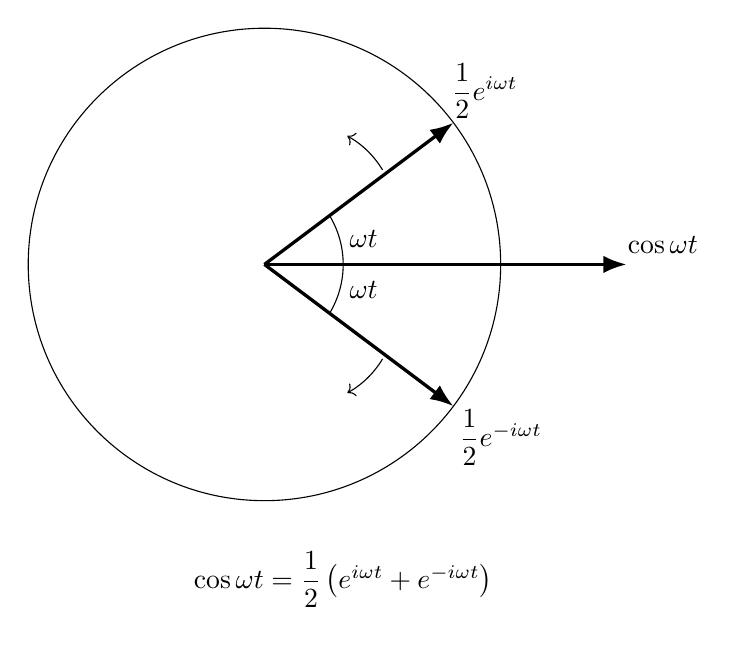
\begin{tikzpicture}[scale=2,
		vector/.style={-{Latex}, very thick}]

        \draw (0, 0) circle (1.5cm);
        \draw [vector] (0, 0) -- (2.3, 0) node[above, pos=1.1] {$\cos \omega t$};
        \draw [vector] (0, 0) -- (1.2, 0.9);
        \node at (1.4, 1.1) {$\dfrac{1}{2} e^{i \omega t}$};
        \draw [vector] (0, 0) -- (1.2, -0.9);
        \node at (1.5, -1.1) {$\dfrac{1}{2} e^{-i \omega t}$};

        \draw (0.5, 0) arc(0:31:0.6) node [midway, right] {$\omega t$};
        \draw (0.5, 0) arc(0:-31:0.6) node [midway, right] {$\omega t$};
        \draw [->] (0.75, 0.6) arc (31:61:0.6);
        \draw [->] (0.75, -0.6) arc (-31:-61:0.6);

        \node at (0.5, -2) {$\cos \omega t = \dfrac{1}{2} \left( e^{i \omega t}  + e^{- i \omega t} \right)$};

\end{tikzpicture}
\end{document}